\chapter{Manual de instalación}
\label{ch:manual_instalacion}

Puesto que la publicación de la aplicación en un mercado de aplicaciones no entra dentro del alcance del desarrollo, la única instalación posible es por medio de la \acrshort{apk}. Este fichero se puede obtener entre los archivos adjuntos a este documento o se puede descargar en el apartado \textbf{Releases}\footnote{\href{https://github.com/kriogenia/AllForOne-App/releases}{https://github.com/kriogenia/AllForOne-App/releases}} del repositorio público de GitHub: 

\begin{figure}[H]
    \centering
    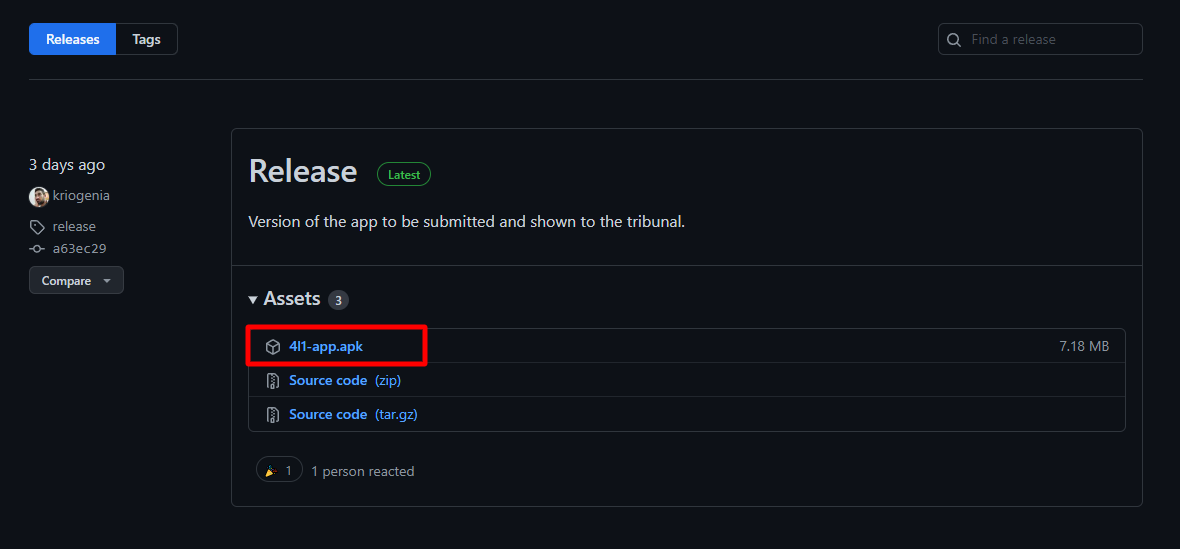
\includegraphics[width=1\textwidth]{Manuales/ManualInstalacion.png}
    \caption{Descarga de la APK desde el repositorio}
    \label{man:instalacion}
\end{figure}

Una vez se tenga el archivo \code{.apk} este deberá ser transferido al dispositivo móvil en el que se quiera instalar. También es posible descargar la \acrshort{apk} desde el propio \emph{smartphone} en el link anterior. Al no ser una aplicación descargada desde un \emph{marketplace} certificado será necesario habilitar la instalación de aplicaciones de orígenes desconocidos en los \textbf{Ajustes} del sistema\cite{xatakaApk}.

Tras activar dicho permiso el fichero podrá ser abierto desde el gestor de ficheros del sistema operativo. Si Android pregunta si estás seguro de realizar la instalación, confirma que sí. Cuando la instalación finalice la aplicación ya estará lista para ser usada. \emph{Véase \fref{ch:manual_usuario} \nameref{ch:manual_usuario}}.